\section{Photosensors}

\subsection{Superlattice deposition}

Typical large area APDs have poor quantum efficiency in the BaF$_2$ spectral region.  However, APDs and SiPMs/MPPCs from Hamamatsu and RMD made without the normal protective epoxy coating, and therefore somewhat fragile,  have quantum efficiencies in the 200 nm region of ~17\%~\cite{sato:2013}. These devices cannot, however, discriminate between the 220 nm fast component and 300 nm slow components of BaF$_2$. The presence of the slow component limits the rate capability of the calorimeter, and can therefore be an issue in high background conditions.

Our approach is to transform a large-area (9$\times$9 mm$^2$) RMD APD~\cite{RMD}, which has high gain (up to 2000) and low capacitance 0.7pf/mm$^2$, into a superlattice-doped APD~\cite{hoenk:2013} and to incorporate an atomic layer deposition (ALD) antireflection filter~\cite{hennessy:2015} that provides ~60\% quantum efficiency at 220 nm and ~0.1\% efficiency at 300 nm, thereby enabling us to obtain a larger number of photoelectrons/MeV, and also to take full advantage of the fast decay time component of BaF$_2$.

Superlattice (2D) doping, a JPL-developed surface passivation technique, produces stable surfaces on silicon photosensors. These techniques were developed to overcome surface damage due to ultraviolet radiation in satellite instrumentation. The subsurface structures are formed using a combination of molecular beam epitaxy and controlled crystalline silicon growth. After growing a thin layer of undoped silicon, a monolayer of boron is deposited, then another silicon layer is grown, and the process is repeated up to four times. The resulting subsurface structure, with high quality self-organized layers of boron atoms at densities of $\sim\!\! 2\times 10^{14}/{\rm cm}^2$ (see Figure~\ref{fig:delta}),

\begin{figure}[h!]
\centering
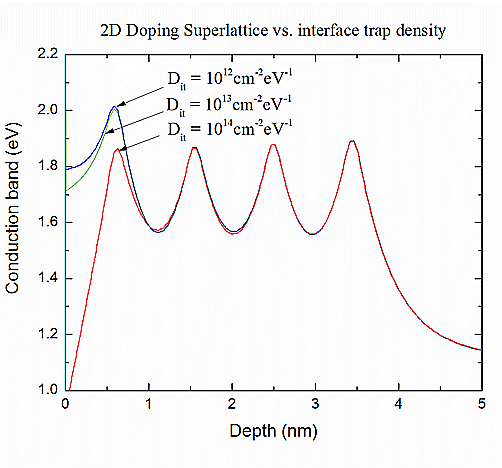
\includegraphics[width=0.9\linewidth]{Figures/delta.png}
\caption{A four-layer superlattice grown by MBE, in
which four 2D-doped layers are separated by 1 nm. This 2D doping creates a maximum field of 10$^7$ V/cm. The 2D doping superlattice forms a surface
depletion layer with a fixed width of less than 1 nm, which is stable against interface trap densities in excess of
10$^{14}$ cm$^{-3}$, enabling the detector to remain stable even when the surface is severely damaged by irradiation by DUV radiation. }
\label{fig:delta}
\end{figure}
\begin{figure}[h!]
\centering
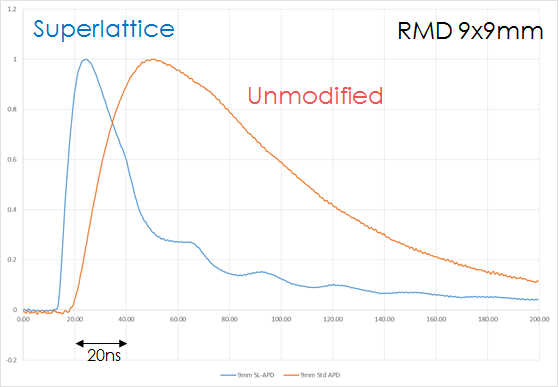
\includegraphics[width=0.9\linewidth]{Figures/timing.png}
\caption{Response of unmodified and superlattice-doped 9$\times$9 mm$^2$ RMD APDs. }
\label{fig:timing}
\end{figure}

The reason for the low QE achieved by most solid state devices in the UV region is two-fold: in typical devices there is an undepleted region of tens of microns between the Si/SiO$_2$ passivation region on the absorbing surface and the depletion region that is in close proximity to the avalanche region.
Due to quantum exclusion, the superlattice structure suppresses recombination of charge at the surface, thereby improving the QE in the 220 nm region to close to the theoretical maximum. The greatly reduced undepleted region of the superlattice-doped device also produces substantially improved timing characteristics (see Figure~\ref{fig:timing}). Second, most devices have a protective resin layer that lowers the net quantum efficiency. This layer is not required in our device, which is passivated and protected by the creation of an atomic layer deposition filter described below.

\subsection{Atomic layer deposition filter}

It then remains to apply a multilayered atomic layer deposition (ALD) coating to serve as a bandwidth-reducing interference and antireflection filter.  These films, in our case alternating layers of aluminum and aluminum oxide, are created by forming a series of single atomic layers through self-limiting chemical reactions with the substrate. This process produces uniform pinhole-free layers of precise thickness. Figure~\ref{fig:filter} shows the calculated transmission of such a filter as a function of wavelength. For a five-layer ALD coating, the QE at normal incidence for the fast component of BaF$_2$ is close to 70\%, and the extinction at the slow component wavelength is nearly complete. The transmission of the interference filter is a function of incident angle, which is shown in Figure~\ref{fig:angle}.



\begin{figure}[h!]
\centering
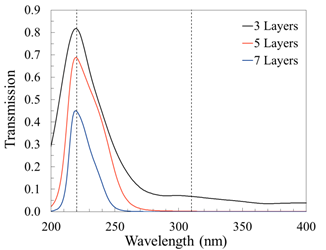
\includegraphics[width=0.9\linewidth]{Figures/filter1.png}
\caption{Quantum efficiency (QE) as a function of wavelength for  three, five seven layer ALD filters. }
\label{fig:filter}
\end{figure}

\begin{figure}[h!]
\centering
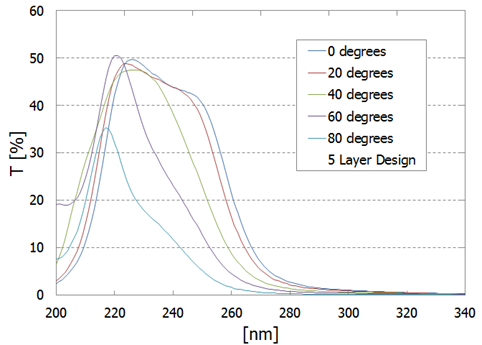
\includegraphics[width=0.9\linewidth]{Figures/angle.png}
\caption{Angular response of the five layer ALD filter as a function of wavelength.}
\label{fig:angle}
\end{figure}


\section{Electrical performance}

We have produced several versions of superlattice/ALD-modified RMD APDs thus far. The anticipated filter response and quantum efficiency improvements have been experimentally demonstrated. The devices, however, have somewhat elevated dark current and noise, as seen in Figure~\ref{fig:noise}. Operation at somewhat reduced temperatures improves the noise performance substantially: at $\sim\!\! 25^\circ$ below ambient, the noise of the superlattice/ALD-modified devices is equivalent to that of standard devices at room temperature.

Several process variations are being investigated to reduce the dark current and associated noise. These include variation of the parameters of the superlattice deposition layers, modification of the first dielectric layer of the ALD filter and changes to the electrical contact geometry. The current devices are nonetheless suitable for deployment in the Mu2e calorimeter.

\begin{figure}[h!]
\centering
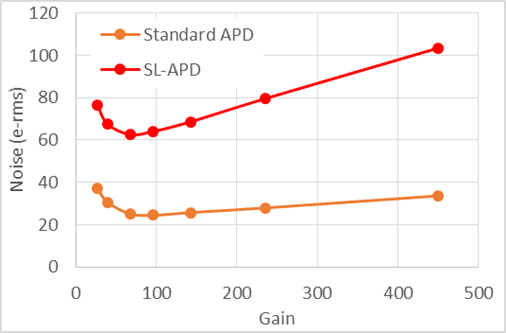
\includegraphics[width=0.9\linewidth]{Figures/noise.png}
\caption{Noise in {\t rms} electrons of a standard and a superlattice-doped RMD APD as a function of gain.}
\label{fig:noise}
\end{figure}



\begin{figure}[h!]
\begin{center}
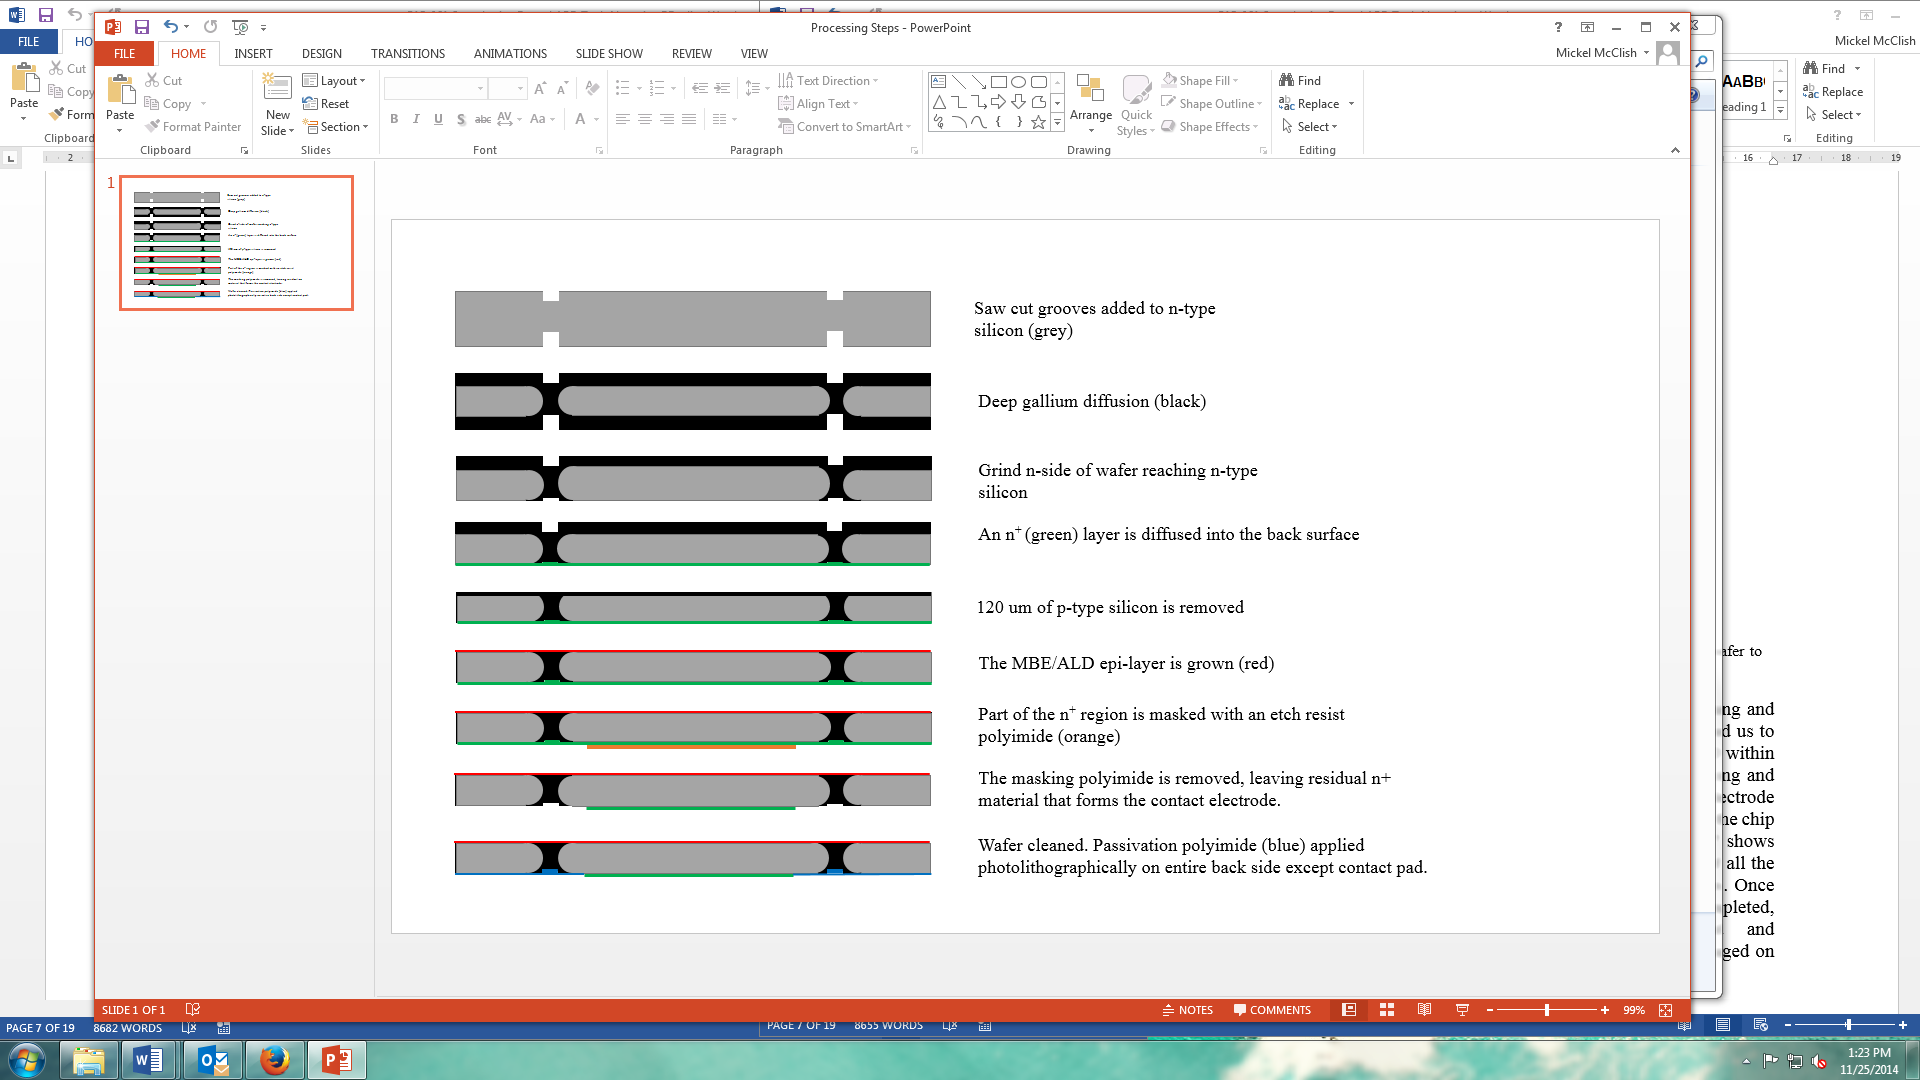
\includegraphics[width=0.7\columnwidth]{Figures/RMD_process.png}
\caption{Replace this text with your caption.}
\end{center}
\end{figure}

\begin{figure}[h!]
\begin{center}
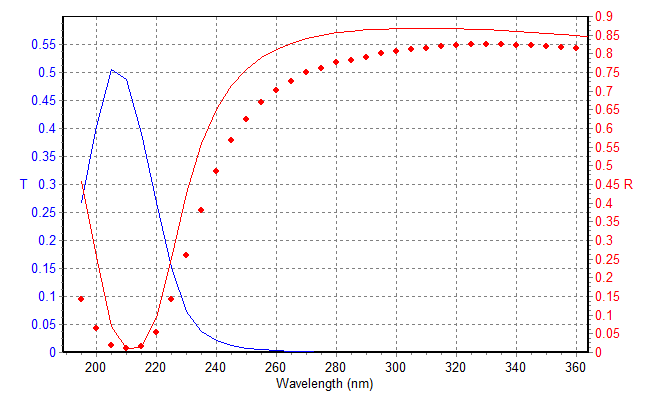
\includegraphics[width=0.7\columnwidth]{Figures/fivelayer.png}
\caption{Calculated response of five layer ALD filter.}
\end{center}
\end{figure}
